% Options for packages loaded elsewhere
\PassOptionsToPackage{unicode}{hyperref}
\PassOptionsToPackage{hyphens}{url}
\documentclass[
]{article}
\usepackage{xcolor}
\usepackage[margin=1in]{geometry}
\usepackage{amsmath,amssymb}
\setcounter{secnumdepth}{5}
\usepackage{iftex}
\ifPDFTeX
  \usepackage[T1]{fontenc}
  \usepackage[utf8]{inputenc}
  \usepackage{textcomp} % provide euro and other symbols
\else % if luatex or xetex
  \usepackage{unicode-math} % this also loads fontspec
  \defaultfontfeatures{Scale=MatchLowercase}
  \defaultfontfeatures[\rmfamily]{Ligatures=TeX,Scale=1}
\fi
\usepackage{lmodern}
\ifPDFTeX\else
  % xetex/luatex font selection
\fi
% Use upquote if available, for straight quotes in verbatim environments
\IfFileExists{upquote.sty}{\usepackage{upquote}}{}
\IfFileExists{microtype.sty}{% use microtype if available
  \usepackage[]{microtype}
  \UseMicrotypeSet[protrusion]{basicmath} % disable protrusion for tt fonts
}{}
\makeatletter
\@ifundefined{KOMAClassName}{% if non-KOMA class
  \IfFileExists{parskip.sty}{%
    \usepackage{parskip}
  }{% else
    \setlength{\parindent}{0pt}
    \setlength{\parskip}{6pt plus 2pt minus 1pt}}
}{% if KOMA class
  \KOMAoptions{parskip=half}}
\makeatother
\usepackage{color}
\usepackage{fancyvrb}
\newcommand{\VerbBar}{|}
\newcommand{\VERB}{\Verb[commandchars=\\\{\}]}
\DefineVerbatimEnvironment{Highlighting}{Verbatim}{commandchars=\\\{\}}
% Add ',fontsize=\small' for more characters per line
\usepackage{framed}
\definecolor{shadecolor}{RGB}{248,248,248}
\newenvironment{Shaded}{\begin{snugshade}}{\end{snugshade}}
\newcommand{\AlertTok}[1]{\textcolor[rgb]{0.94,0.16,0.16}{#1}}
\newcommand{\AnnotationTok}[1]{\textcolor[rgb]{0.56,0.35,0.01}{\textbf{\textit{#1}}}}
\newcommand{\AttributeTok}[1]{\textcolor[rgb]{0.13,0.29,0.53}{#1}}
\newcommand{\BaseNTok}[1]{\textcolor[rgb]{0.00,0.00,0.81}{#1}}
\newcommand{\BuiltInTok}[1]{#1}
\newcommand{\CharTok}[1]{\textcolor[rgb]{0.31,0.60,0.02}{#1}}
\newcommand{\CommentTok}[1]{\textcolor[rgb]{0.56,0.35,0.01}{\textit{#1}}}
\newcommand{\CommentVarTok}[1]{\textcolor[rgb]{0.56,0.35,0.01}{\textbf{\textit{#1}}}}
\newcommand{\ConstantTok}[1]{\textcolor[rgb]{0.56,0.35,0.01}{#1}}
\newcommand{\ControlFlowTok}[1]{\textcolor[rgb]{0.13,0.29,0.53}{\textbf{#1}}}
\newcommand{\DataTypeTok}[1]{\textcolor[rgb]{0.13,0.29,0.53}{#1}}
\newcommand{\DecValTok}[1]{\textcolor[rgb]{0.00,0.00,0.81}{#1}}
\newcommand{\DocumentationTok}[1]{\textcolor[rgb]{0.56,0.35,0.01}{\textbf{\textit{#1}}}}
\newcommand{\ErrorTok}[1]{\textcolor[rgb]{0.64,0.00,0.00}{\textbf{#1}}}
\newcommand{\ExtensionTok}[1]{#1}
\newcommand{\FloatTok}[1]{\textcolor[rgb]{0.00,0.00,0.81}{#1}}
\newcommand{\FunctionTok}[1]{\textcolor[rgb]{0.13,0.29,0.53}{\textbf{#1}}}
\newcommand{\ImportTok}[1]{#1}
\newcommand{\InformationTok}[1]{\textcolor[rgb]{0.56,0.35,0.01}{\textbf{\textit{#1}}}}
\newcommand{\KeywordTok}[1]{\textcolor[rgb]{0.13,0.29,0.53}{\textbf{#1}}}
\newcommand{\NormalTok}[1]{#1}
\newcommand{\OperatorTok}[1]{\textcolor[rgb]{0.81,0.36,0.00}{\textbf{#1}}}
\newcommand{\OtherTok}[1]{\textcolor[rgb]{0.56,0.35,0.01}{#1}}
\newcommand{\PreprocessorTok}[1]{\textcolor[rgb]{0.56,0.35,0.01}{\textit{#1}}}
\newcommand{\RegionMarkerTok}[1]{#1}
\newcommand{\SpecialCharTok}[1]{\textcolor[rgb]{0.81,0.36,0.00}{\textbf{#1}}}
\newcommand{\SpecialStringTok}[1]{\textcolor[rgb]{0.31,0.60,0.02}{#1}}
\newcommand{\StringTok}[1]{\textcolor[rgb]{0.31,0.60,0.02}{#1}}
\newcommand{\VariableTok}[1]{\textcolor[rgb]{0.00,0.00,0.00}{#1}}
\newcommand{\VerbatimStringTok}[1]{\textcolor[rgb]{0.31,0.60,0.02}{#1}}
\newcommand{\WarningTok}[1]{\textcolor[rgb]{0.56,0.35,0.01}{\textbf{\textit{#1}}}}
\usepackage{graphicx}
\makeatletter
\newsavebox\pandoc@box
\newcommand*\pandocbounded[1]{% scales image to fit in text height/width
  \sbox\pandoc@box{#1}%
  \Gscale@div\@tempa{\textheight}{\dimexpr\ht\pandoc@box+\dp\pandoc@box\relax}%
  \Gscale@div\@tempb{\linewidth}{\wd\pandoc@box}%
  \ifdim\@tempb\p@<\@tempa\p@\let\@tempa\@tempb\fi% select the smaller of both
  \ifdim\@tempa\p@<\p@\scalebox{\@tempa}{\usebox\pandoc@box}%
  \else\usebox{\pandoc@box}%
  \fi%
}
% Set default figure placement to htbp
\def\fps@figure{htbp}
\makeatother
\setlength{\emergencystretch}{3em} % prevent overfull lines
\providecommand{\tightlist}{%
  \setlength{\itemsep}{0pt}\setlength{\parskip}{0pt}}
\usepackage[]{natbib}
\bibliographystyle{plainnat}
\usepackage{bookmark}
\IfFileExists{xurl.sty}{\usepackage{xurl}}{} % add URL line breaks if available
\urlstyle{same}
\hypersetup{
  pdftitle={HW 03 - Road traffic accidents},
  pdfauthor={Tina Huynh},
  hidelinks,
  pdfcreator={LaTeX via pandoc}}

\title{HW 03 - Road traffic accidents}
\author{Tina Huynh}
\date{}

\begin{document}
\maketitle

{
\setcounter{tocdepth}{2}
\tableofcontents
}
\begin{figure}
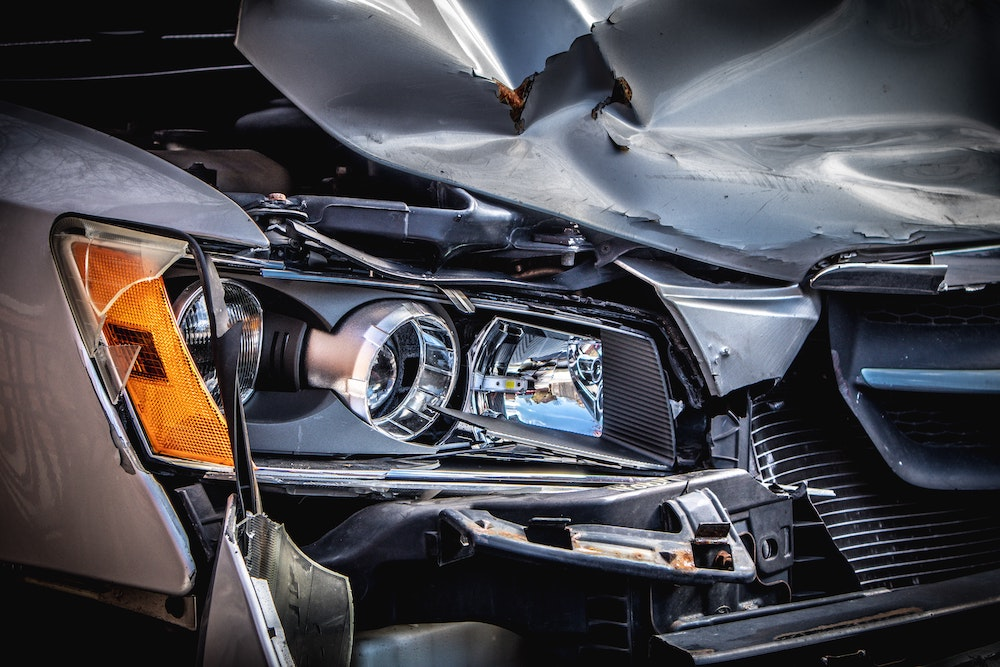
\includegraphics[width=0.8\linewidth]{img/accident} \caption{Photo by Clark Van Der Beken on Unsplash}\label{fig:photo}
\end{figure}

In this assignment we'll look at traffic accidents in Edinburgh. The
data are made available
\href{https://data.gov.uk/dataset/cb7ae6f0-4be6-4935-9277-47e5ce24a11f/road-safety-data/datafile/36f1658e-b709-47e7-9f56-cca7aefeb8fe/preview}{online}
by the UK Government. It covers all recorded accidents in Edinburgh in
2018 and some of the variables were modified for the purposes of this
assignment.

\section{Getting started}\label{getting-started}

\textbf{IMPORTANT:} If there is no GitHub repo created for you for this
assignment, it means I didn't have your GitHub username as of when I
assigned the homework. Please let me know your GitHub username asap, and
I can create your repo.

Go to the course GitHub organization and locate your homework repo,
which should be named \texttt{hw-03-YOUR\_GITHUB\_USERNAME}. Grab the
URL of the repo, and clone it in RStudio. First, open the R Markdown
document \texttt{hw-03.Rmd} and Knit it. Make sure it compiles without
errors. The output will be in the file markdown \texttt{.md} file with
the same name.

\subsection{Warm up}\label{warm-up}

Before we introduce the data, let's warm up with some simple exercises.

\begin{itemize}
\tightlist
\item
  Update the YAML, changing the author name to your name, and
  \textbf{knit} the document.
\item
  Commit your changes with a meaningful commit message.
\item
  Push your changes to GitHub.
\item
  Go to your repo on GitHub and confirm that your changes are visible in
  your Rmd \textbf{and} md files. If anything is missing, commit and
  push again.
\end{itemize}

\subsection{Packages}\label{packages}

We'll use the \textbf{tidyverse} package for much of the data wrangling
and visualization and the data lives in the \textbf{dsbox} package.
These packages are already installed for you. You can load them by
running the following in your Console:

\begin{Shaded}
\begin{Highlighting}[]
\FunctionTok{library}\NormalTok{(tidyverse)}
\FunctionTok{library}\NormalTok{(dsbox)}
\end{Highlighting}
\end{Shaded}

\subsection{Data}\label{data}

The data can be found in the \textbf{dsbox} package, and it's called
\texttt{accidents}. Since the dataset is distributed with the package,
we don't need to load it separately; it becomes available to us when we
load the package. You can find out more about the dataset by inspecting
its documentation, which you can access by running \texttt{?accidents}
in the Console or using the Help menu in RStudio to search for
\texttt{accidents}. You can also find this information
\href{https://rstudio-education.github.io/dsbox/reference/accidents.html}{here}.

\section{Exercises}\label{exercises}

\begin{enumerate}
\def\labelenumi{\arabic{enumi}.}
\tightlist
\item
  How many observations (rows) does the dataset have? Instead of hard
  coding the number in your answer, use inline code.
\end{enumerate}

The dataset contains 768 observations.

\textbf{Tired of typing your password?} Chances are your browser has
already saved your password, but if not, you can ask Git to save (cache)
your password for a period of time, where you indicate the period of
time in seconds. For example, if you want it to cache your password for
1 hour, that would be 3,600 seconds. To do so, run the following
\emph{in the Console}:
\texttt{usethis::use\_git\_config(credential.helper\ =\ "cache\ -\/-timeout=3600")}.
If you want to cache it for a longer time, you can adjust the number of
seconds in the code.

\begin{enumerate}
\def\labelenumi{\arabic{enumi}.}
\setcounter{enumi}{1}
\tightlist
\item
  Run \texttt{View(accidents)} in your Console to view the data in the
  data viewer. What does each row in the dataset represent?
\end{enumerate}

Each row in the dataset represents a distinct traffic accident that
occurred in Edinburgh in 2018. Each accident entry includes detailed
information about the time and location of the incident, weather and
road conditions at the time, the severity of the accident, and various
characteristics of the vehicles and casualties involved.

🧶 ✅ ⬆️ Knit, \emph{commit, and push your changes to GitHub with an
appropriate commit message. Make sure to commit and push all changed
files so that your Git pane is cleared up afterwards.}

\begin{enumerate}
\def\labelenumi{\arabic{enumi}.}
\setcounter{enumi}{2}
\tightlist
\item
  Recreate the following plot, and describe in context of the data. In
  your answer, don't forget to label your R chunk as well (where it says
  \texttt{label-me-1}). Your label should be short, informative,
  shouldn't include spaces, and shouldn't shouldn't repeat a previous
  label.
\end{enumerate}

\begin{Shaded}
\begin{Highlighting}[]
\NormalTok{accidents }\SpecialCharTok{\%\textgreater{}\%}
  \FunctionTok{mutate}\NormalTok{(}\AttributeTok{day\_of\_week\_type =} \FunctionTok{if\_else}\NormalTok{(day\_of\_week }\SpecialCharTok{\%in\%} \FunctionTok{c}\NormalTok{(}\StringTok{"Saturday"}\NormalTok{, }\StringTok{"Sunday"}\NormalTok{), }\StringTok{"Weekend"}\NormalTok{, }\StringTok{"Weekday"}\NormalTok{)) }\SpecialCharTok{\%\textgreater{}\%}
  \FunctionTok{ggplot}\NormalTok{(}\FunctionTok{aes}\NormalTok{(}\AttributeTok{x =}\NormalTok{ time, }\AttributeTok{fill =}\NormalTok{ severity)) }\SpecialCharTok{+}
  \FunctionTok{geom\_density}\NormalTok{(}\AttributeTok{alpha =} \FloatTok{0.5}\NormalTok{) }\SpecialCharTok{+}
  \FunctionTok{facet\_wrap}\NormalTok{(}\SpecialCharTok{\textasciitilde{}}\NormalTok{day\_of\_week\_type, }\AttributeTok{ncol =} \DecValTok{1}\NormalTok{) }\SpecialCharTok{+}
  \FunctionTok{theme\_minimal}\NormalTok{() }\SpecialCharTok{+}
  \FunctionTok{scale\_fill\_viridis\_d}\NormalTok{() }\SpecialCharTok{+}
  \FunctionTok{labs}\NormalTok{(}
    \AttributeTok{title =} \StringTok{"Number of accidents throughout the day"}\NormalTok{,}
    \AttributeTok{subtitle =} \StringTok{"By day of week and severity"}\NormalTok{,}
    \AttributeTok{x =} \StringTok{"Time of day"}\NormalTok{,}
    \AttributeTok{y =} \StringTok{"Density"}\NormalTok{,}
    \AttributeTok{fill =} \StringTok{"Severity"}
\NormalTok{  )}
\end{Highlighting}
\end{Shaded}

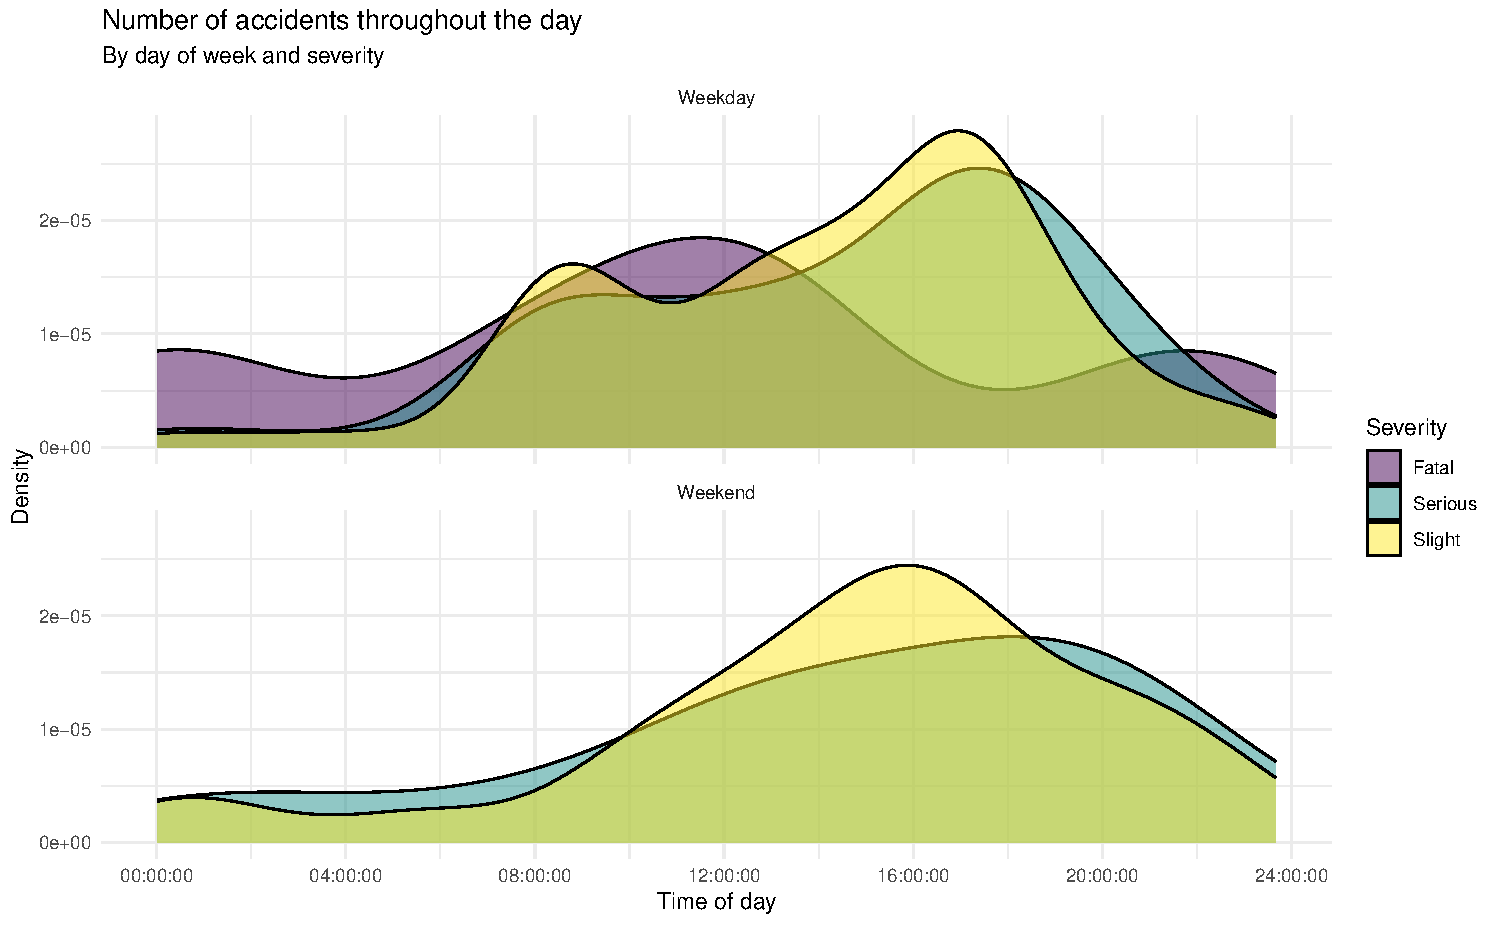
\includegraphics[width=0.8\linewidth]{hw-03-accidents_files/figure-latex/time_severity_plot-1}

The density plot above reveals critical temporal patterns in Edinburgh's
traffic accidents, comparing weekday and weekend incidents by time of
day and severity.

On weekdays, the data shows two prominent accident peaks: one during the
morning rush hour (approximately 8-9 AM) and a larger, more sustained
peak during the afternoon/evening commute (3-6 PM). This bimodal
distribution strongly correlates with typical commuting patterns,
suggesting that traffic congestion during work commutes significantly
contributes to accident frequency. Notably, the afternoon peak is more
pronounced and extends over a longer period, potentially reflecting the
less synchronized nature of evening commutes compared to morning ones.

Weekend accident patterns differ substantially, with accidents more
evenly distributed throughout the day and reaching their highest
frequency in the afternoon and early evening hours. The absence of a
morning peak on weekends reflects the reduced early-day traffic when
commuting pressures are absent. Instead, the gradual increase in
accidents throughout the day likely corresponds to increased leisure
travel, shopping activities, and potentially social events later in the
day.

Regarding severity, ``Slight'' accidents (indicated in purple)
constitute the majority of incidents across both weekday and weekend
periods. However, ``Serious'' accidents (shown in green-blue) maintain a
relatively consistent proportion throughout the day. Fatal accidents,
while rare, do not show a clear temporal pattern in this visualization,
which is expected given their fortunately infrequent occurrence.

The overall lower density of weekend accidents compared to weekday
incidents suggests that commuter traffic significantly influences
accident rates in Edinburgh. This comprehensive temporal analysis
provides valuable insights for traffic management authorities, who might
consider targeted safety measures during high-risk periods, particularly
weekday commuting hours when accident densities reach their peak.

🧶 ✅ ⬆️ Knit, \emph{commit, and push your changes to GitHub with an
appropriate commit message. Make sure to commit and push all changed
files so that your Git pane is cleared up afterwards.}

\begin{enumerate}
\def\labelenumi{\arabic{enumi}.}
\setcounter{enumi}{3}
\tightlist
\item
  Create another data visualization based on these data and interpret
  it. You can choose any variables and any type of visualization you
  like, but it must have at least three variables, e.g.~a scatterplot of
  x vs.~y isn't enough, but if points are colored by z, that's fine. In
  your answer, don't forget to label your R chunk as well (where it says
  \texttt{label-me-2}).
\end{enumerate}

\begin{Shaded}
\begin{Highlighting}[]
\CommentTok{\# First, examine the speed limit and weather distributions}
\NormalTok{accidents }\SpecialCharTok{\%\textgreater{}\%}
  \FunctionTok{count}\NormalTok{(speed\_limit) }\SpecialCharTok{\%\textgreater{}\%}
  \FunctionTok{arrange}\NormalTok{(}\FunctionTok{desc}\NormalTok{(n))}
\end{Highlighting}
\end{Shaded}

\begin{verbatim}
## # A tibble: 6 x 2
##   speed_limit     n
##         <dbl> <int>
## 1          20   379
## 2          30   246
## 3          40    64
## 4          70    47
## 5          50    19
## 6          60    13
\end{verbatim}

\begin{Shaded}
\begin{Highlighting}[]
\NormalTok{accidents }\SpecialCharTok{\%\textgreater{}\%}
  \FunctionTok{count}\NormalTok{(weather) }\SpecialCharTok{\%\textgreater{}\%}
  \FunctionTok{arrange}\NormalTok{(}\FunctionTok{desc}\NormalTok{(n))}
\end{Highlighting}
\end{Shaded}

\begin{verbatim}
## # A tibble: 9 x 2
##   weather                     n
##   <fct>                   <int>
## 1 Fine + no high winds      618
## 2 Raining + no high winds    65
## 3 Unknown                    29
## 4 Other                      15
## 5 Fine + high winds          14
## 6 Raining + high winds       13
## 7 Snowing + no high winds    11
## 8 Snowing + high winds        2
## 9 Fog or mist                 1
\end{verbatim}

\begin{Shaded}
\begin{Highlighting}[]
\CommentTok{\# Filter out the very infrequent categories for clearer visualization}
\NormalTok{accidents\_filtered }\OtherTok{\textless{}{-}}\NormalTok{ accidents }\SpecialCharTok{\%\textgreater{}\%}
  \FunctionTok{filter}\NormalTok{(weather }\SpecialCharTok{\%in\%} \FunctionTok{c}\NormalTok{(}\StringTok{"Fine + no high winds"}\NormalTok{, }\StringTok{"Raining + no high winds"}\NormalTok{, }\StringTok{"Fine + high winds"}\NormalTok{, }\StringTok{"Raining + high winds"}\NormalTok{)) }\SpecialCharTok{\%\textgreater{}\%}
  \FunctionTok{mutate}\NormalTok{(}
    \AttributeTok{weather\_type =} \FunctionTok{case\_when}\NormalTok{(}
      \FunctionTok{str\_detect}\NormalTok{(weather, }\StringTok{"Fine"}\NormalTok{) }\SpecialCharTok{\textasciitilde{}} \StringTok{"Fine"}\NormalTok{,}
      \FunctionTok{str\_detect}\NormalTok{(weather, }\StringTok{"Rain"}\NormalTok{) }\SpecialCharTok{\textasciitilde{}} \StringTok{"Rainy"}\NormalTok{,}
      \ConstantTok{TRUE} \SpecialCharTok{\textasciitilde{}}\NormalTok{ weather}
\NormalTok{    ),}
    \AttributeTok{wind\_condition =} \FunctionTok{if\_else}\NormalTok{(}\FunctionTok{str\_detect}\NormalTok{(weather, }\StringTok{"high winds"}\NormalTok{), }\StringTok{"High winds"}\NormalTok{, }\StringTok{"No high winds"}\NormalTok{),}
    \AttributeTok{speed\_category =} \FunctionTok{case\_when}\NormalTok{(}
\NormalTok{      speed\_limit }\SpecialCharTok{\textless{}=} \DecValTok{20} \SpecialCharTok{\textasciitilde{}} \StringTok{"20 mph or less"}\NormalTok{,}
\NormalTok{      speed\_limit }\SpecialCharTok{\textless{}=} \DecValTok{30} \SpecialCharTok{\textasciitilde{}} \StringTok{"30 mph"}\NormalTok{,}
\NormalTok{      speed\_limit }\SpecialCharTok{\textless{}=} \DecValTok{40} \SpecialCharTok{\textasciitilde{}} \StringTok{"40 mph"}\NormalTok{,}
      \ConstantTok{TRUE} \SpecialCharTok{\textasciitilde{}} \StringTok{"\textgreater{}40 mph"}
\NormalTok{    ),}
    \AttributeTok{speed\_category =} \FunctionTok{factor}\NormalTok{(speed\_category, }\AttributeTok{levels =} \FunctionTok{c}\NormalTok{(}\StringTok{"20 mph or less"}\NormalTok{, }\StringTok{"30 mph"}\NormalTok{, }\StringTok{"40 mph"}\NormalTok{, }\StringTok{"\textgreater{}40 mph"}\NormalTok{))}
\NormalTok{  )}

\CommentTok{\# Create visualization of weather conditions, speed limits, and accident severity}
\FunctionTok{ggplot}\NormalTok{(accidents\_filtered, }\FunctionTok{aes}\NormalTok{(}\AttributeTok{x =}\NormalTok{ speed\_category, }\AttributeTok{fill =}\NormalTok{ severity)) }\SpecialCharTok{+}
  \FunctionTok{geom\_bar}\NormalTok{(}\AttributeTok{position =} \StringTok{"fill"}\NormalTok{) }\SpecialCharTok{+}
  \FunctionTok{facet\_grid}\NormalTok{(weather\_type }\SpecialCharTok{\textasciitilde{}}\NormalTok{ wind\_condition) }\SpecialCharTok{+}
  \FunctionTok{scale\_fill\_viridis\_d}\NormalTok{() }\SpecialCharTok{+}
  \FunctionTok{theme\_minimal}\NormalTok{() }\SpecialCharTok{+}
  \FunctionTok{labs}\NormalTok{(}
    \AttributeTok{title =} \StringTok{"Proportion of Accident Severity by Speed Limit and Weather Conditions"}\NormalTok{,}
    \AttributeTok{subtitle =} \StringTok{"Edinburgh Traffic Accidents, 2018"}\NormalTok{,}
    \AttributeTok{x =} \StringTok{"Speed Limit Category"}\NormalTok{,}
    \AttributeTok{y =} \StringTok{"Proportion of Accidents"}\NormalTok{,}
    \AttributeTok{fill =} \StringTok{"Accident Severity"}
\NormalTok{  ) }\SpecialCharTok{+}
  \FunctionTok{theme}\NormalTok{(}
    \AttributeTok{axis.text.x =} \FunctionTok{element\_text}\NormalTok{(}\AttributeTok{angle =} \DecValTok{45}\NormalTok{, }\AttributeTok{hjust =} \DecValTok{1}\NormalTok{),}
    \AttributeTok{plot.title =} \FunctionTok{element\_text}\NormalTok{(}\AttributeTok{face =} \StringTok{"bold"}\NormalTok{),}
    \AttributeTok{panel.grid.major.x =} \FunctionTok{element\_blank}\NormalTok{(),}
    \AttributeTok{legend.position =} \StringTok{"bottom"}
\NormalTok{  )}
\end{Highlighting}
\end{Shaded}

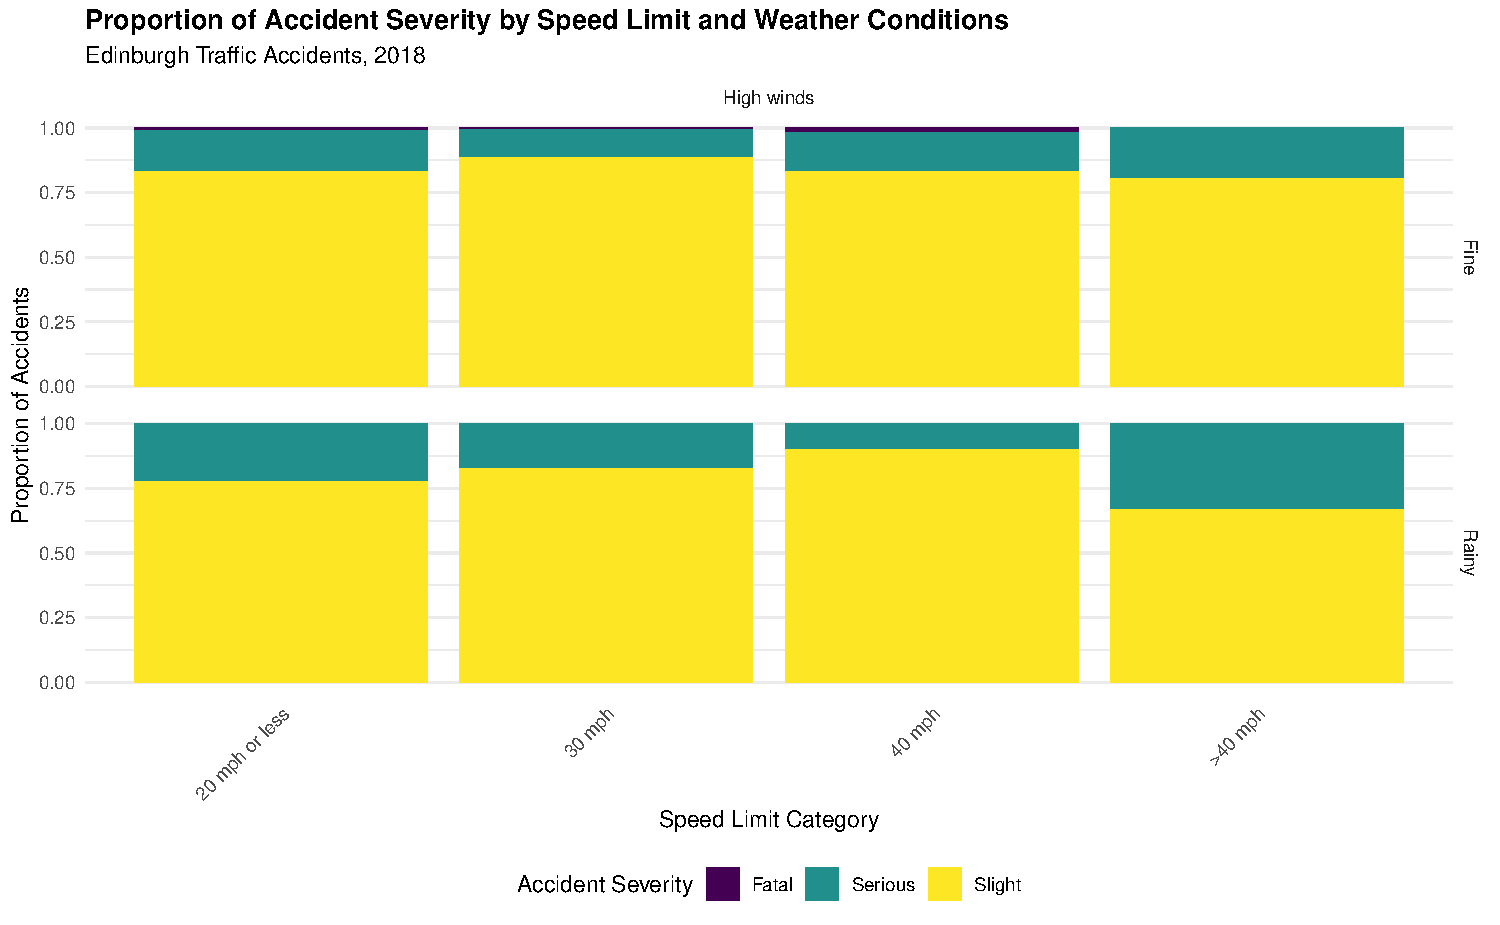
\includegraphics[width=0.8\linewidth]{hw-03-accidents_files/figure-latex/weather_speed_severity-1}

This visualization examines the relationship between speed limits,
weather conditions, and accident severity in Edinburgh's 2018 traffic
incidents, revealing several noteworthy patterns with significant road
safety implications.

The analysis reveals that roads with higher speed limits consistently
demonstrate greater proportions of serious and fatal accidents across
all weather conditions. This progressive relationship is particularly
evident in the 40 mph and \textgreater40 mph categories, where the
proportion of severe outcomes increases substantially compared to
lower-speed zones. This pattern aligns with established traffic safety
principles that higher speeds generate greater kinetic energy during
collisions, resulting in more severe injuries.

Weather conditions exhibit a complex influence on accident severity.
Fine weather without high winds shows relatively consistent severity
distributions across speed categories, likely reflecting ``baseline''
accident patterns. However, the introduction of high winds significantly
alters this pattern, particularly in higher speed zones. In 40 mph zones
during fine weather with high winds, the proportion of serious accidents
increases noticeably compared to the same speed zones without high
winds. This suggests that wind conditions may compromise vehicle
stability or driver control, especially at higher speeds.

Rainy conditions demonstrate an interesting pattern: they generally show
higher proportions of slight accidents in the 30 mph zones compared to
fine weather. This counterintuitive finding may reflect adaptive
behavior, where drivers exercise greater caution during visible adverse
conditions, potentially reducing accident severity despite increased
occurrence. However, when rain combines with high winds in 20 mph or
less zones, we observe a notably higher proportion of serious accidents,
indicating that this combination of adverse conditions may be
particularly hazardous in city centers and residential areas with lower
speed limits.

The data shows few fatal accidents across all categories, making pattern
identification difficult for this severity level. However, their
relative absence in the 20 mph or less zones across all weather
conditions reinforces the safety benefits of lower urban speed limits.

These findings have significant implications for traffic management
policy. They suggest that speed limit reductions could be particularly
beneficial during adverse weather conditions, and that warning systems
for high wind conditions might be especially important on higher-speed
roadways. The data also supports the continued implementation of 20 mph
zones in urban areas, which consistently show the lowest proportion of
serious and fatal accidents across all weather conditions analyzed.

🧶 ✅ ⬆️ Knit, \emph{commit, and push your changes to GitHub with an
appropriate commit message. Make sure to commit and push all changed
files so that your Git pane is cleared up afterwards and review the md
document on GitHub to make sure you're happy with the final state of
your work.} Once you decide that you are done with the lab, choose the
knit drop down and select \texttt{Knit\ to\ tufte\_handout} to generate
a pdf. Download and submit that pdf to Canvas.

\end{document}
